% LTeX: language=it
\documentclass[a4paper, 12pt, Arial]{article}

%\usepackage{mathrsfs}
\usepackage{amssymb}
\usepackage{amsmath}
\usepackage{array}
\usepackage{epsfig}
\usepackage{float}
\usepackage[margin=2cm]{geometry}
%\usepackage[sectionbib]{chapterbib}
\usepackage{fancyhdr}
\usepackage{lastpage}
\usepackage{graphicx}
\usepackage{caption}
\usepackage{subcaption}
\usepackage{array}
\usepackage{amsfonts}
%\usepackage{color}
\usepackage[usenames,dvipsnames]{color}
\usepackage[hyperindex, linktocpage]{hyperref}
\usepackage[italian]{babel}
\usepackage{wrapfig}
% \renewcommand{\rmdefault}{phv} % Arial
% \renewcommand{\sfdefault}{phv} % Arial

%%%%%%%%%%%%%%%%%%%%%%%%%%%%%%
\newcommand{\class}{Laboratorio di Automatica}
\newcommand{\expT}{Controllo PI di un motore CC}
\newcommand{\repN}{1}
\newcommand{\stud}{Lorenzo Franceschetti, 2000263\\ Leonardo Luigi Pepe, 2009734\\ Federico Saporiti, 2000264}
\newcommand{\dateD}{29 Maggio 2023}

% \renewcommand{\textheight}{710pt}
% \renewcommand{\topmargin}{-12pt}

% - Introduzione: modellare motore dc per poi controllarlo con PI
% - Lab 5: modellazione e PI dato
% - Lab 6: calcolo coefficienti PI da specifiche
% - Lab Sperimentale 1: Verifica comportamento

\begin{document}

%\renewcommand{\baselinestretch}{1.5}

\begin{center}
\begin{tabular}{| p{\textwidth} |}
    \hline
    \large
    \vspace{-2pt}
    \stud \hfill
    \Large
    \begin{center}
    {\color{BrickRed}
        \textsl{\class}\\
        \textsl{Relazione n.\repN: \expT}\\
        \large
        \dateD}
    \vspace{-4mm}
    \end{center}\\
    \hline
\end{tabular}
\end{center}

\section{Introduzione}
\subsection{Scopo dell'attività}
L'obiettivo è quello di creare un modello, tramite MatLab e Simulink, di un motore in cc e di progettare un controllore PI rispettando delle specifiche assegnate, in modo da poter controllare la velocità del motore, per poi verificare sperimentalmente in laboratorio che il comportamento reale del motore sia congruo a quello atteso.
\subsection{Organizzazione della relazione}
La relazione si divide in 3 parti: nella prima si crea il modello Simulink del motore in modo da poter eseguire le simulazioni necessarie per verificare il comportamento del controllore prima di applicarlo al motore reale. Questo modello viene poi retroazionato applicando un controllore P e successivamente PI, in modo da evidenziarne il diverso comportamento e valutare la tipologia migliore da usare. Nella seconda parte, invece, partendo da delle specifiche nel dominio del tempo del sistema in catena chiusa, si ricavano i parametri del controllore da usare per il controllo in velocità del motore, con seguente verifica sul modello precedentemente sviluppato. Infine, nell'ultima parte, si procede alla verifica sperimentale del comportamento del controllore, usando Simulink in tempo reale per controllare il motore elettrico fornito in laboratorio.

\section{Modellazione del motore tramite Simulink}
\subsection{Disegno del modello}
Partendo dalle equazioni che regolano la dinamica elettrica e meccanica del motore, sia dal punto di vista del motore che da quello del carico, si può ricavare un modello del sistema implementabile tramite Simulink. Nel disegnare lo schema, si è tenuto conto delle non idealità del driver di tensione del motore e del convertitore analogico-digitale, come saturazione e quantizzazione. Per la misura della velocità, si è implementato un sistema composto da tre diversi filtri, uno a tempo continuo del primo ordine, uno a tempo continuo del secondo ordine e uno a tempo discreto. Il programma permette di selezionare quale dei tre usare per calcolare la velocità a partire dalla lettura dell'angolo. In questo modo è possibile valutare quale dei tre fornisce il dato più vicino a quello reale, sia in termini di media che di varianza. Per la risoluzione delle equazioni, si è fatto ricorso a un metodo a passo variabile per la soluzione numerica delle equazioni differenziali che regolano il modello, in particolare si è scelto il metodo $ode45$.
\begin{figure}[H]
    \centering
    \begin{subfigure}{0.3\linewidth}
        \centering
        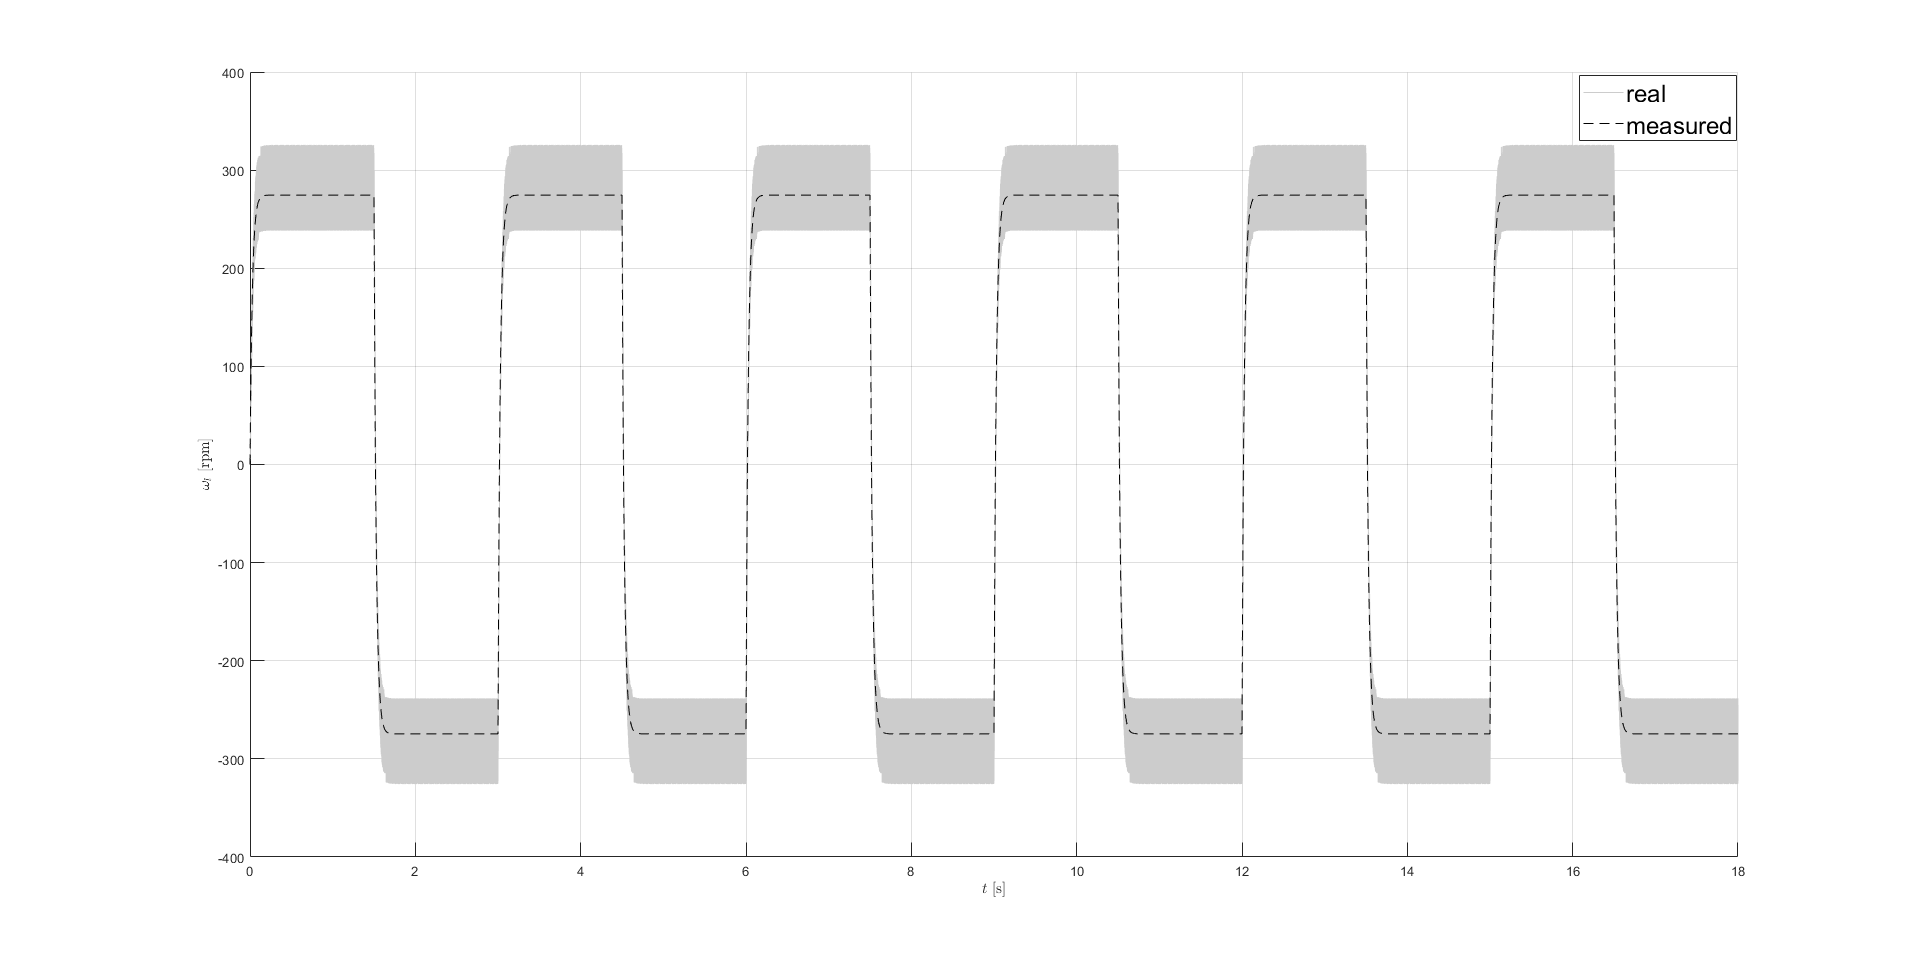
\includegraphics[width=\linewidth]{./Images/speed_filter_1.png}
        \caption{Filtro a tempo continuo del primo ordine}
        \label{Lab5:first}
    \end{subfigure}
    \begin{subfigure}{0.3\linewidth}
        \centering
        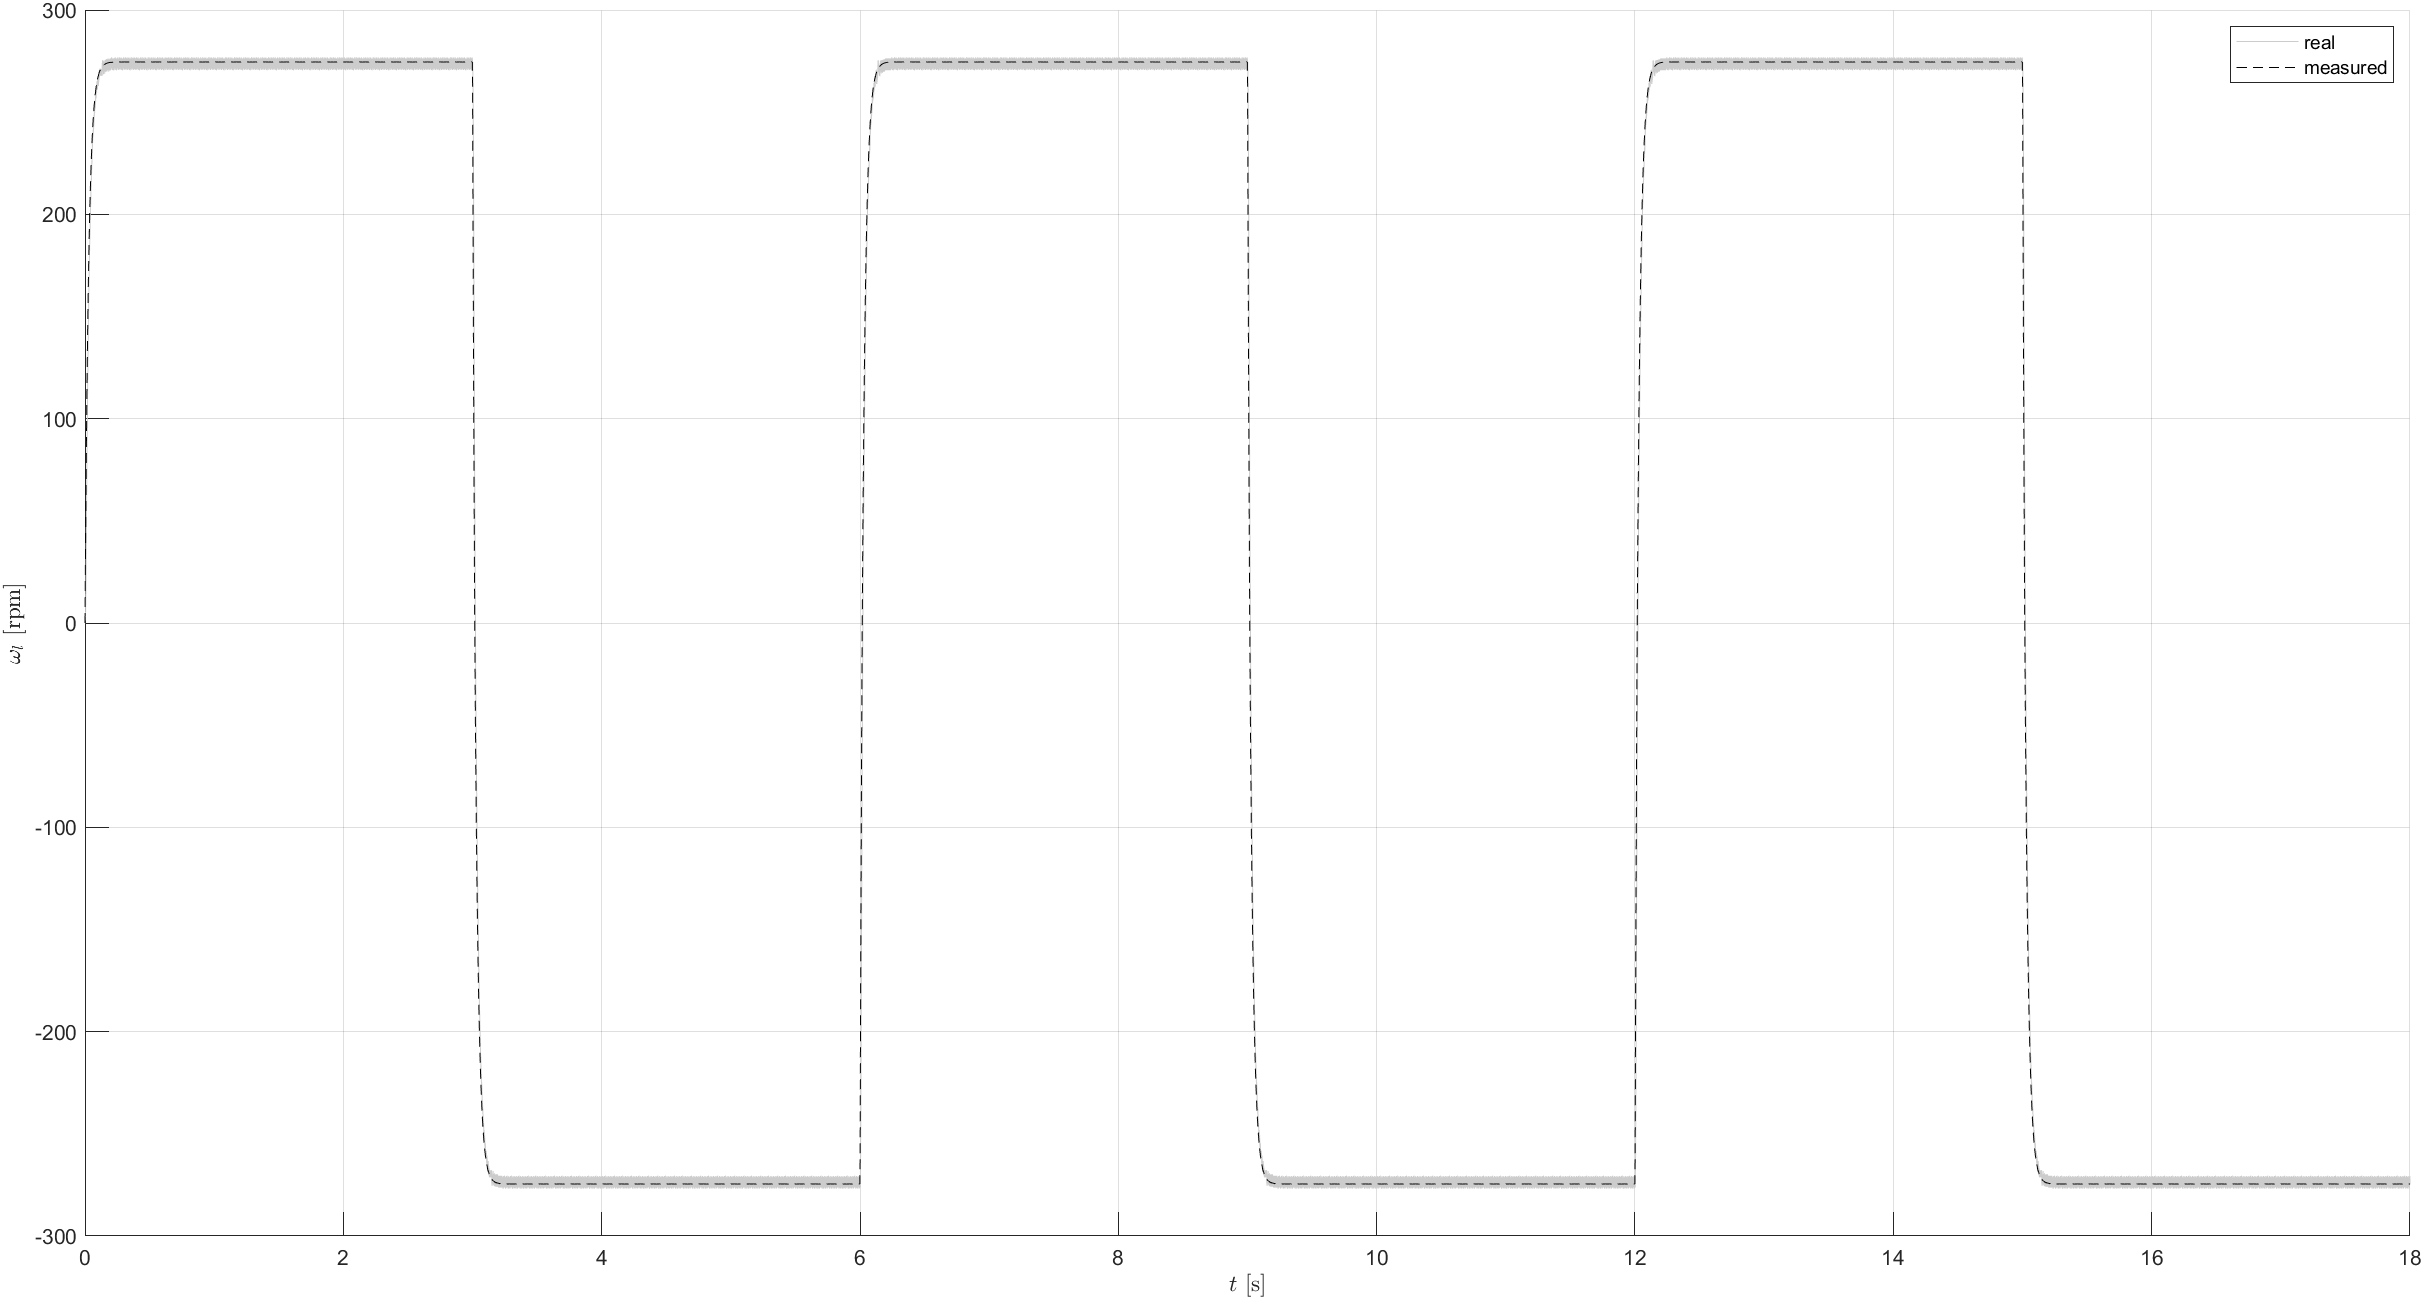
\includegraphics[width=\linewidth]{./Images/speed_filter_2.png}
        \caption{Filtro a tempo continuo del secondo ordine}
        \label{Lab5:second}
    \end{subfigure}
    \begin{subfigure}{0.3\linewidth}
        \centering
        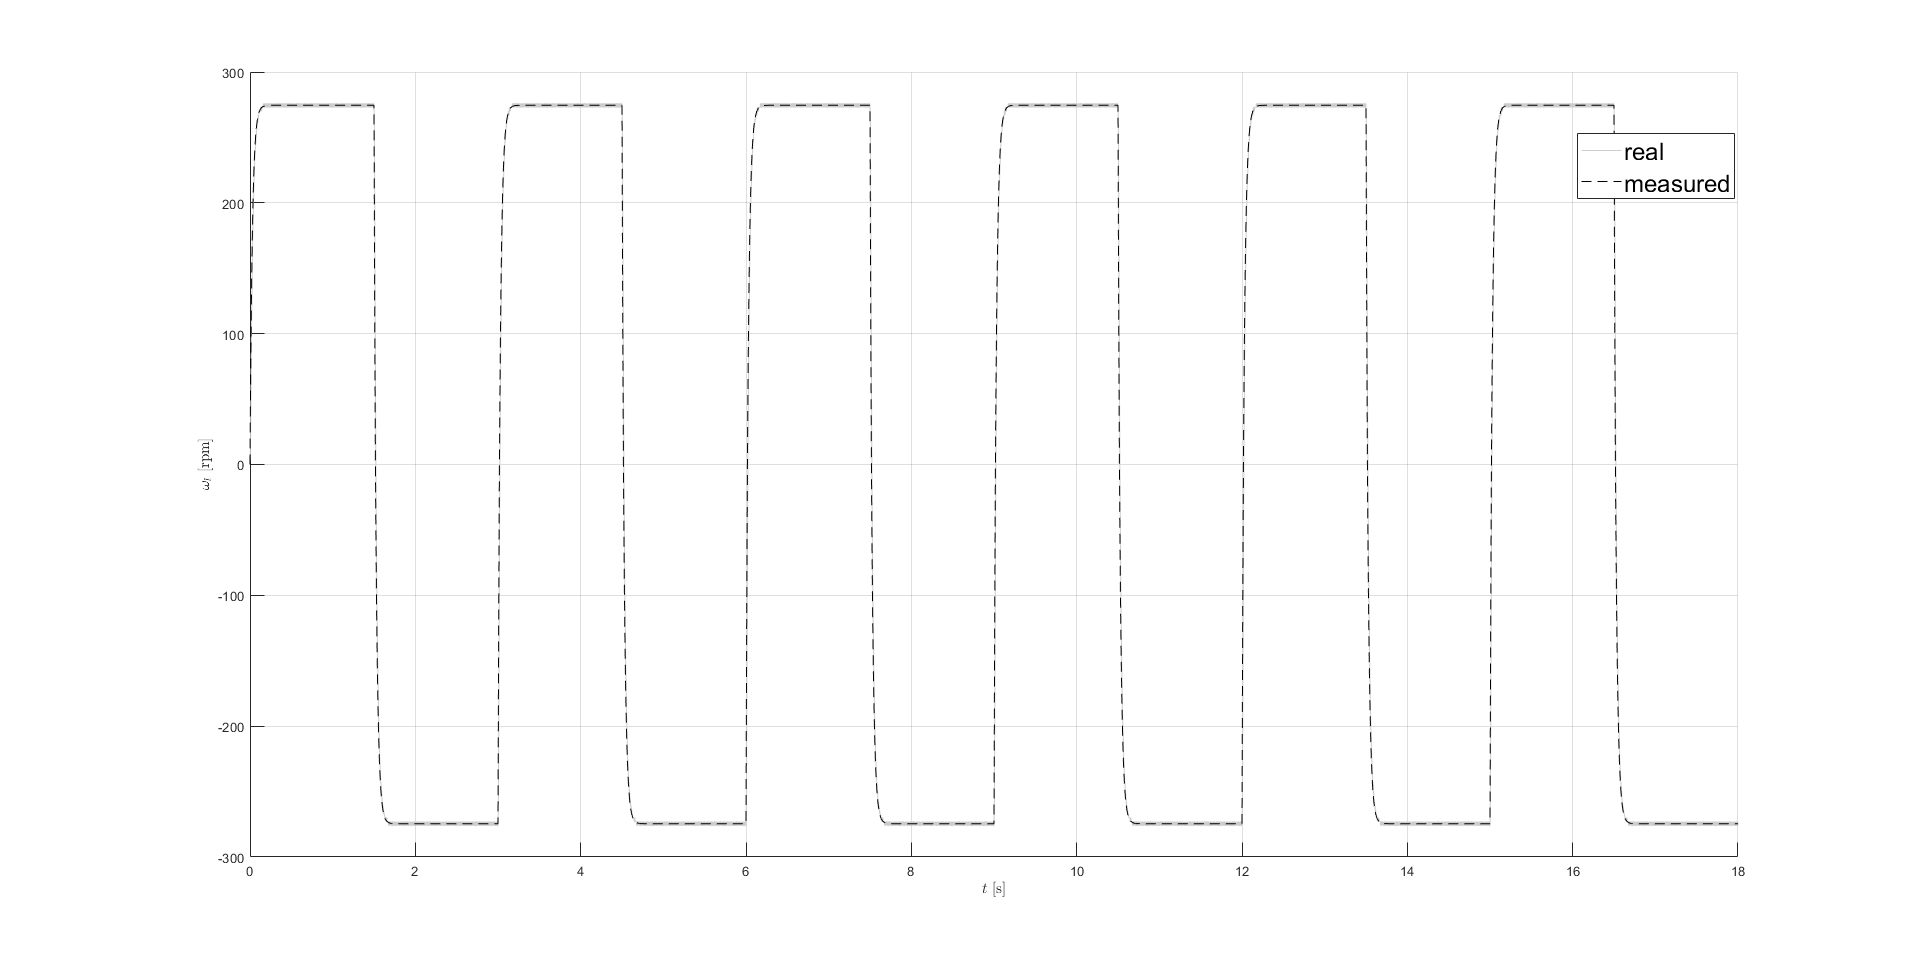
\includegraphics[width=\linewidth]{./Images/speed_filter_3.png}
        \caption{Filtro discreto del decimo ordine}
        \label{Lab5:discrete}
    \end{subfigure}
    \caption{Simulazione velocità}
\end{figure}

\begin{wrapfigure}{r}{0.5\textwidth}
  \begin{center}
    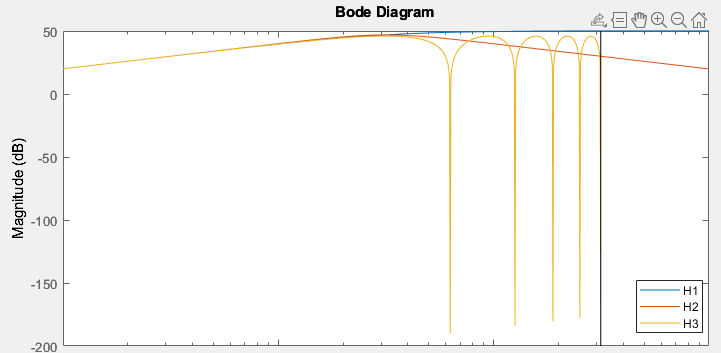
\includegraphics[width=0.45\textwidth]{./Images/speed_filter_responses.png}
  \end{center}
  \caption{Modulo FDT}
  \label{Lab5:mags}
\end{wrapfigure}

Si nota come il filtro del primo ordine dia un risultato molto rumoroso rispetto agli altri due. Infatti, come si ricava dalla figura \ref{Lab5:mags}, il filtro del primo ordine ha modulo quasi costante ad alte pulsazioni, pari a $50 dB$, mentre gli altri due hanno modulo decrescente e quindi riescono a attenuare in maniera più efficiente i disturbi alle alte frequenze, dando un risultato meno rumoroso.

\subsection{Controllo in retroazione di velocità}
Per fare in modo che il motore segua in maniera corretta un segnale di riferimento di velocità, è possibile sfruttare la retroazione con un controllore adeguato, che permetta al sistema di inseguire un segnale costante con errore nullo a regime.

\section{Progettazione controllore PI}
\subsection{}
\section{Verifica sperimentale del comportamento del controllore}
\subsection{}
\end{document}
